\documentclass[12pt]{article}
\usepackage{mandi}
\usepackage{braket}
\usepackage{graphicsx}
\usepackage{amsmath}
\usepackage{amsfonts}
\usepackage{tikz}
\usepackage{epstopdf}
\tolerance=1
\emergencystretch=\maxdimen
\hyphenpenalty=10000
\hbadness=10000
% Palatino font (ppl must be installed).
%\renewcommand*\rmdefault{ppl}
% Iwona font (iwona must be installed).
%\renewcommand*\rmdefault{iwona}
\begin{document}
\title{Principles Of Economics Notebook}
\author{Anurag Pallaprolu}
\maketitle
\begin{enumerate}
\item Anything \textbf{marginal} is always some change upon some other change. Hence, it is usually related to \textit{differentiation of the quantity whose marginal value is to be found}. For example
$$MP_L = \frac{\Delta Total Product}{\Delta Labour}$$
\textbf{Marginal Product} is hence, \textit{the slope of the Total Product curve.}
\item Anything \textbf{average} is by definition, the straightforward ratio. For example
$$AP_L = \frac{Total Product}{Labour}$$
\item For a \textbf{household case}, there always exists a \textbf{budget constraint}, which is
$$Income = XP_X + YP_Y$$
The general idea of a \textbf{utility maximization of income} is done when the following condition holds, in the case of two products X and Y:
$$\frac{MU_X}{P_X} = \frac{MU_Y}{P_Y}$$
Here, it is very clear that, the marginal utility is defined, as pointed before, the slope of the utility function and according to the \textbf{law of diminishing utility} the slope is usually a decreasing function.
\item \textbf{The income effect}:  Consumption changes because purchasing power changes.
\textbf{The substitution effect}:  Consumption changes because opportunity costs change. Hence, in the case of income effect, when a product is cheaper, a person will buy it with respect to his income, now \textit{relatively} higher, whereas in the case of the substitution effect, if the product gets cheaper, it will be more preferred when compared to its competitors. \textbf{Consumer surplus} is the difference between the maximum amount a person is willing to pay for a good and its current market price. It is the area on the price-quantity curve between the amount willing to be paid and the price or more mathematically
$$CS = \int_{Price_{Willing}}^{Eq Price} PdQ$$
\item When we look at \textbf{firms} we usually talk about \textbf{costs} and \textbf{revenues}. The standard equation is given by 
$$TC = TFC + TVC$$
It is again clear, what expression to expect for Average Variable Cost $$AVC = \frac{TVC}{q}$$
and the Marginal Cost is the same as the Marginal Variable Cost as the TFC has a zero derivative.
$$MC = \frac{dTVC}{dq}$$ The interesting point to be noted is that \textbf{the point where the average variable cost curve intersects the \textit{rising} MC curve, it is the minimum of the AVC curve}. Mathematically
$$AVC = MC $$$$ \frac{dMC}{dq} > 0$$
$$\frac{dAVC}{dq} = 0$$
all occur simultaneously.
\item The definition of average total cost is simply $$ATC = \frac{TC}{q} = \frac{TFC}{q} + \frac{TVC}{q}$$ Another simple fact to remember is a recall of the previous point that the MC curve will intersect the AVC and ATC curves \textbf{both} at their point of minima.
\item The total revenue generated by any firm is simply 
$$TR = Price*quantity$$
The marginal revenue is simply by definition, 
$$MR = \frac{dTR}{dq}$$ In a \textbf{perfect competition}, the price of a product is kept constant at \textbf{equilibrium}, then
$$MR = \frac{Pdq}{dq} = P$$
\item The \textbf{profit maximizing condition} for all  \textbf{output markets} is the point where $$MC = MR$$ or
$$\frac{dTC}{dq} = \frac{dTR}{dq}$$ In a perfect market, we have seen in the previous point, the MR is the equilibrium price and hence, 
$$P = MC = MR$$ is the profit maximization condition. \textit{The key idea here is that firms will produce as long as marginal revenue exceeds marginal cost.}
\item The \textbf{operating profit} of a firm is given by the equation $$OP = TR - TVC$$
If revenues \textit{exceed} variable costs, operating profit is positive and \textbf{can be used to offset fixed costs and reduce losses, and it will pay the firm to keep operating.}
The important fact that must be noted here is the different decisions a firm can take to survive or shutdown. It is \textit{profitable} for a firm to operate at a \textbf{lower price than equilibrium} if $$TVC<TR<TC$$ than to shutdown completely as the previous condition saves some amount to overcome the variable costs and hence, the net loss suffered is \textbf{lesser} when compared to the shutdown condition.

It is \textit{profitable} for a company to \textbf{shutdown} than operate at prices lesser than equilibrium when the following condition exists 
$$TR<TVC<TC$$
as in this case, the loss suffered due to \textbf{just the fixed costs} is much better than the overhead added by operating and incurring variable losses.

\textbf{The lowest point on the AVC curve, or, from the fact mentioned before, the point of intersection of AVC and MC is the \textit{shutdown point} of a firm.} That is, if the equilibrium condition falls to this point, it is better to shutdown than incur short run losses.

\item A \textbf{scale of economy or diseconomy} is a short-run decision case which need not necessarily represent the actual scenario. The \textbf{Long Run Average Cost curve LRAC is the envelope curve that wraps around all such scaled markets or short-run decision curves}. The image should clarify.
\begin{center}
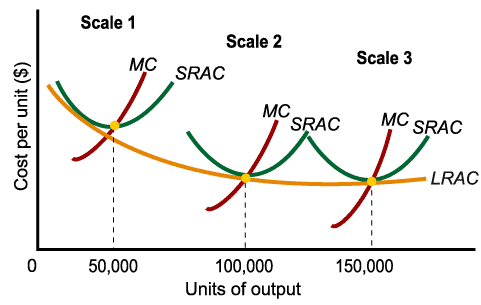
\includegraphics[scale=0.9]{lrac.png}
\end{center}
The various predictions that can be made regarding a given market is that \textbf{firms will enter the market as long as they scale along the \textit{downward sloping part} of the LRAC and they will exit the market once the scaling is along the \textit{upward sloping part} of the LRAC}.

The optimal scale of plant is the scale that \textbf{minimizes average cost}.
\begin{center}
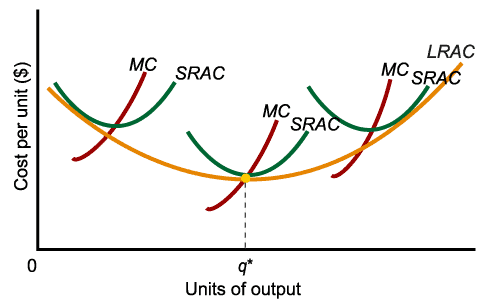
\includegraphics[scale=0.5]{lracscale.png}
\end{center}
Ultimately, the \textbf{profit maximization rule for long run decisions} is given by $$P^* = MC_{Short Run} = AC_{Short Run} = LC_{Long Run}$$
\item We redefine the \textbf{marginal product of labor} as 
$$MP_L = \frac{dP}{dL}$$ When we want to calculate the revenue product of any quantity, we have to multiply it by the price per quantity, in this case the \textbf{marginal product of labor} is given by
$$MRP_L = MP_L*P_X$$

\textbf{\textit{One Variable Factor} Firms will use that factor as long as its marginal revenue product exceeds its unit cost.
} This general statement can be specified for the case of labor being the one variable, in this case, as long as the $$MRP_L \geq W^*$$ where $W^*$ is the current \textbf{wage rate per day per labourer}. The image given below is of infinite importance, as it combines both the viewpoints of costs and labour in markets as two sides of the same coin
\begin{center}
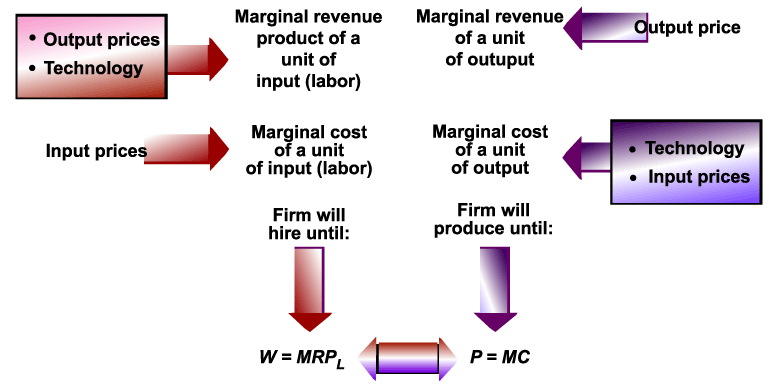
\includegraphics[scale=0.5]{mrplmc.png}
\end{center}
\item Firms generally try to maximize their given income utilization function, in this case it consists of two variables \textbf{labour(L) and capital(K)}. The \textbf{factor substitution effect} takes place when a \textbf{capital intensive} firm looks to become \textbf{labour intensive} to reduce the cost of the unit and vice versa. The income utility function takes the form of $$I = P_LL+P_KK$$
Also, \textbf{Output effect of a factor price increase}: When a firm decreases (increases) its output in response to a factor price increase (decrease), this decreases (increases) its demand for all factors.
\item Unlike labour and capital, \textbf{land markets} are perfectly inelastic, i.e, \textbf{there is a fixed supply of land(this is the supply curve, a line parallel to y axis) and the price/rent is decided by the demand curve}.
Again, the profit maximization condition for land markets is given by (here A represents acres of land)
$$MRP_A = P_A$$
This along with 
$$P_{Labour} = W^* = MRP_L$$
$$P_{Capital} = MRP_K$$
form a complete set of profit maximising rules, written more succintly as
\begin{center}
\boxed{\frac{MP_L}{P_L} = \frac{MP_K}{P_K} = \frac{MP_A}{P_A} = \frac{1}{P_A}}
\end{center}
\item A few general points regarding the \textbf{distribution of income}. If markets are competitive, the equilibrium price of an input is equal to its marginal revenue product 
At equilibrium, each factor ends up receiving rewards determined by its productivity as measured by its MRP. This is called the \textbf{marginal productivity theory of income distribution}.
\item Capital goods form an important part of the assets,t he important part being \textbf{there is always demand for capital goods irrespective of time dimension}. \textbf{Depreciation} is a decline in an asset's economic value over time (because it wears out or it becomes obsolete). 
A \textbf{bond} is a contract between a borrower and a lender, in which the borrower agrees to pay the loan at some time in the future, along with interest payments along the way.
The \textbf{financial capital market} is the part of the capital market in which savers and investors interact through intermediaries (like banks, insurance companies,etc) that stand between the lender and borrower.
The \textbf{present value of R dollars, t years from now} with a rate of r, is given by 
$$PV = \frac{R}{(1+r)^t}$$
\textbf{Lower} interest rates result in \textbf{higher present} values.  The firm has to pay \textbf{more} now to purchase the \textbf{same} number of future dollars.

\item An \textbf{imperfectly competitive industry} is an industry in which single firms have some control over the price of their output. \textbf{Market power} is defined as the imperfectly competitive firm's ability to raise price without losing all demand for its product.\textbf{Monopoly} is defined to be an industry with a single firm in which entry of new firms is blocked. \textbf{Oligopoly} is defined as an industry in which there is a small number of firms , each large enough to have an impact on market price of the output.
The \textbf{ease} with which \textbf{consumers} can substitute for a product \textbf{limits the extent to which a monopolist can exercise market power}.

\item There are many things which prevent firms from entering into the industry, for instance, \textbf{governmental directives such as laws placed on the sale of a particular product} help the industry which is \textbf{already} selling the product by setting up a monopoly. Similarly, \textbf{patents} also lead to such biasing towards the inventor and firms have to pay \textbf{royalty} to him/her/the inventor's firm. Thirdly, A \textbf{large initial investment}, or the need to embark in an \textbf{expensive advertising campaign}, deter would-be entrants to the industry. Ownership of a scarce factor of production also helps in setting up a barrier on new entrants. 
\item In perfect competition, demand curve is a horizontal line; marginal revenue is equal to price of output. However, in a monopolistic market, there is \textbf{no difference between a firm and the industry}. Monopoly faces a \textbf{known demand curve}, i.e., firm has enough information to predict how households will react to different price. The \textbf{demand curve} facing a perfectly competitive firm is perfectly elastic; \textbf{in a monopoly, the market demand curve is the demand curve facing the firm and the total quantity supplied in the market is what the monopoly firm decides to produce}.
\item There are many features to detect a monopoly, At every level of output except one unit, \textbf{a monopolist's marginal revenue is below price}. A monopoly firm has no supply curve that is independent of the demand curve for its product. Even monopolists can run out of business if they cannot catch up with the running costs and the expected overhead. Hence, similar profit maximizing rules can be applied here too, that is 
$$MR = MC$$ is the profit maximizing condition.
\item \textbf{Collusion} is the act of working with other producers in an effort to limit competition and increase joint profits. When firms collude, the outcome would be exactly the same as the outcome of a monopoly in the industry.
\item There are problems with monopolistic economy. Monopoly leads to an \textbf{inefficient mix of output}. Price is above marginal cost, which means that the firm is \textbf{underproducing} from society's point of view.

\item There can be many remedies for monopoly developing in economies. The involvement of \textbf{governments} in economies is quite contradictory. They try \textbf{promoting} competition by these remedies but again \textbf{restrict} markets with \textbf{industrial rules}. We shall look at a few commissions and acts one by one.
\item \textbf{Interstate Commerce Commission (ICC)}:  A federal regulatory group created by Congress in 1887 to oversee and correct abuses in the railroad industry.\\
\textbf{Sherman Act} Passed by Congress in 1890, the act declared every contract or conspiracy to restrain trade among states or nations illegal and declared any attempt at monopoly, successful or not, a misdemeanor.  Interpretation of which specific behaviors were legal fell to the courts.\\
\textbf{Clayton Act} Passed by Congress in 1914 to strengthen the Sherman Act and clarify the rule of reason, the act outlawed specific monopolistic behaviors such as tying contracts, price discrimination, and unlimited mergers.\\
\textbf{Federal Trade Commission (FTC)} A federal regulatory group created by Congress in 1914 to investigate the structure and behavior of firms engaging in interstate commerce, to determine what constitutes unlawful “unfair” behavior, and to issue cease-and-desist orders to those found in violation of antitrust law.\\
\textbf{Wheeler-Lea Act (1938)} Extended the language of the Federal Trade Commission Act to include deceptive as well as unfair methods of competition.\\

\item We can introduce variations in monopolistic economies. \textbf{A monopolistically competitive industry has a lot of firms competing, \textit{no barriers to entry} and product differentiation.} Some degree of market power is achieved by firms producing differentiated products.
New firms can enter and established firms can exit such an industry with ease. The only way in which any market power can be gained is by \textbf{differentiation of the product },hence substitution effect and related effects can be observed in such a structure.  Product differentiation can most efficiently be exhibited when \textbf{advertising} is done properly. Product differentiation and advertising \textbf{waste society's scarce resources}, argue critics. They say \textbf{enormous sums of money are spent to create minute, meaningless differences among products}.
\item There is a definite way to detect a monopolistically competitive market by looking at the \textbf{demand curve}. It is \textbf{less elastic than the demand curve faced by a perfectly competitive firm}, but it is likely to be \textbf{more elastic than the demand curve faced by a monopoly}. Even in a monopolistically competitive market, the profit maximizing condition is given by $$MC=MR$$
\item The firm's \textbf{demand curve must end up tangent to its average total cost curve for profits to equal zero}.  This is the condition for long-run equilibrium in a monopolistically competitive industry.
\begin{center}
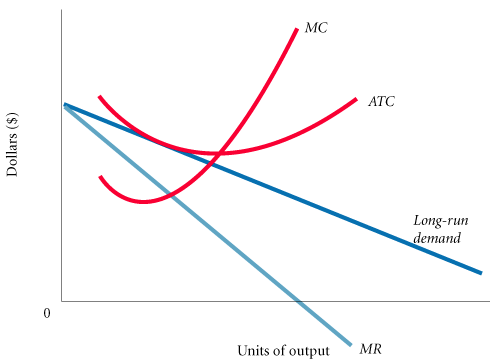
\includegraphics[scale=0.5]{mcflre.png}
\end{center}











\end{enumerate}
\end{document}
